\documentclass[Softwaredesign/Softwaredesign_main.tex]{subfiles}


\begin{document}

\section{GUI layout}
\begin{figure}
    \centering
    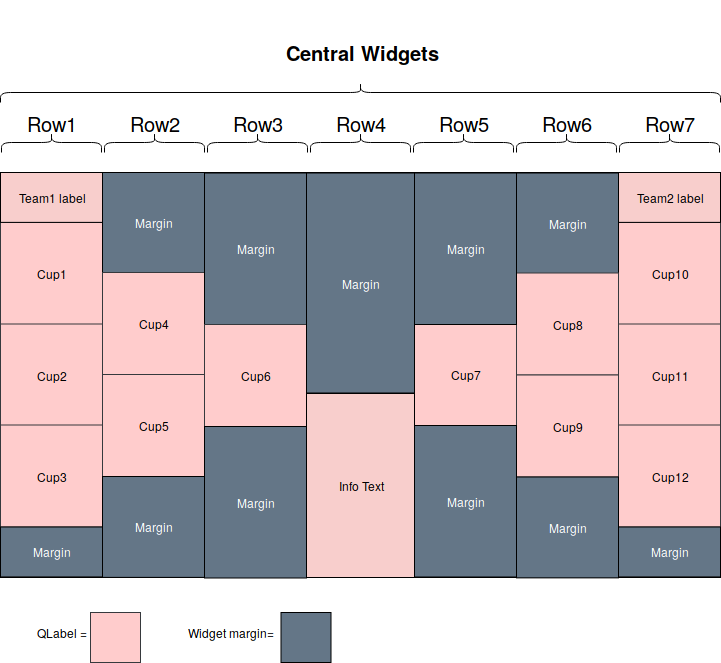
\includegraphics[scale=0.5]{Softwaredesign/GUI/Pictures/Boards_design.png}
    \caption{Visualisering af implementering gui Widgets og Labels}
    \label{gui_design_implementering}
\end{figure}

GUI'en har et fast layout. Dette betyder at labels, widgets osv. ikke bevæger sig i forhold til hinande. Det har fordelen at applikationen vil passe til flere forskellige skærmopløsninger eller vindues størrelser. Dette faste layout opnåes ved at først at "definere" hele programmet; i dette tilfælde ville hele programmet være "Centrel Widget". Central widget ville være der hvor baggrunden ville vises på. Det centrale widget deles derefter op i 7 rækker: Row1-Row7. De her rækker indeholder enten margin, som er tom plads; Derudover indeholder rækkerne også Labels som viser enten tekst eller billeder. Alle rækkerne er delt op i kolonner. I disse kolonner bestemmes størrelsen af "Margin", ellers bestemmes størrelsen af QLabels. Det ses på figur \ref{gui_design_implementering} hvad hver QLabel bliver brugt til, når i brug. Cup1 til og med Cup12 bruges til at vise om en given kop er "on" eller "off". Ellers er der et QLabel som bruges til "info text" som er tekst som anviser hvad brugeren skal gøre for at starte spillet. Disse labels er nødvendigvis ikke synlige, men skal altid logisk gemmes i hukommelsen.

\end{document}